\documentclass[journal]{IEEEtran}
\usepackage{amsmath,amssymb,amsthm}
\usepackage{graphicx}
\usepackage{booktabs}
\usepackage{cite}
\usepackage{url}
\usepackage{xcolor}
\usepackage{microtype}

\newtheorem{proposition}{Proposition}
\newtheorem{theorem}{Theorem}
\newcommand{\ours}{FORTRESS-FL}

\begin{document}

\title{Certified Federated Unlearning for IoT: Ledger-Anchored Revocation with Anytime-Valid Forgetting Certificates}

\author{Quang-Vinh Dang%
\thanks{Q.-V. Dang is with RMIT University Vietnam. E-mail: vinh.dang3@rmit.edu.vn.}%
}

\maketitle

\begin{abstract}
Federated learning lets IoT devices train a shared model without exporting data, but a device's influence stays in the model after it leaves, and regulation, decommissioning and poisoned contributions all demand removal. Retraining for every request is too costly for constrained fleets, and existing federated unlearning checks are empirical, intrusive or limited to logging the request. We present a federated unlearning and governance layer for the FORTRESS-FL robust aggregation system. A hash-chained ledger with Merkle roots, per-round checkpoints of model and reputation state, and a consent registry make revocation traceable. Clients plant paired ghost canaries before training; after a revocation wave an anytime-valid e-process verifier (VOUCH) issues an $(\epsilon,\alpha)$ forgetting certificate without retrained references or backdoor markers. A verify-then-escalate policy tries cheap unlearning operators first and releases the first certified, utility-preserving model, with a proof that the error budget $\alpha$ holds over the whole ladder, and it reports an audit as unpowered when the canaries were not memorised. On a synthetic fleet, on smartphone sensor data (UCI HAR) and on botnet traffic from nine real IoT devices (N-BaIoT), with a linear model and an MLP, exactly retrained models were wrongly flagged in 4 of 280 runs (1.4\%). The ladder certified waves at 31--97\% lower mean client energy than retraining, with a worst case 44\% above it on synthetic data. Batching 20 revocations cut per-client energy 29-fold, and with an MLP on HAR a single client could be certified from 60 canary pairs. Ledger overhead was about 1\% of update traffic.
\end{abstract}

\begin{IEEEkeywords}
Federated unlearning, model governance, provenance, anytime-valid inference, Byzantine robustness, Internet of Things.
\end{IEEEkeywords}

\section{Introduction}
\IEEEPARstart{F}{ederated} learning lets IoT devices train a shared model without exporting raw data~\cite{mcmahan2017}, but a device's data keeps influencing the global model long after the device has left. Data protection law gives owners a right to erasure~\cite{gdpr}, devices are decommissioned or change owner, and poisoned contributions are discovered after the fact. Retraining from scratch for every request costs the whole fleet its original training energy and radio traffic, which is not realistic at IoT scale.

Federated unlearning removes a client's influence without full retraining~\cite{liu2021federaser,halimi2022,wu2022kd,liu2024survey}. Two problems remain for deployment. First, the operator has to \emph{show} that the influence is gone. Existing checks mark the leaving client's data with backdoor-style markers~\cite{gao2024verifi}, rely on fingerprints~\cite{goswami2026}, or record requests on a blockchain~\cite{zuo2024,blockful2024}; the first two are empirical and the third records that unlearning was requested rather than whether it worked. Second, verification is almost never tied to cost: an operator who must pay for a certificate has little reason to choose the cheap method over the expensive one unless the certificate tells them whether the cheap method was enough.

We address both problems in one system built on the \ours{} robust aggregation pipeline~\cite{dang2025fortress} and on the paired-canary verifier VOUCH~\cite{dang2026vouch}. Our contributions are:
\begin{enumerate}
\item \textbf{Ledger-anchored revocation.} A hash-chained provenance ledger with per-round Merkle roots over client updates, a consent registry, and per-round checkpoints of the model \emph{and} of the reputation state, since reputations also remember past contributors. A rollback record names the clean checkpoint, so an auditor can check lineage and bind a certificate to the ledger head and the released model hash.
\item \textbf{Federated paired-canary certificates.} Clients plant paired ghost canaries before training and commit to them in the ledger. After a revocation wave, an anytime-valid e-process verifier~\cite{dang2026vouch} issues or withholds an $(\epsilon,\alpha)$ forgetting certificate. The null is generated by the clients' own coins, so no retrained reference model, shadow models or backdoor markers are needed. We adapt the protocol to client-level revocation, partial participation and batched waves.
\item \textbf{Verify-then-escalate.} A cost ladder from update subtraction to rollback in which the certificate is the acceptance test. We prove that splitting the error budget over the rungs keeps the probability of ever certifying a leaky model below $\alpha$ (Theorem~\ref{thm:esc}), and we add a utility guard because forgetting that destroys the model is not a result.
\item \textbf{Evaluation on resource-constrained fleets.} We quantify client energy and traffic under an explicit cost model, on a synthetic fleet and on real smartphone sensor data (UCI HAR~\cite{anguita2013}) and real IoT botnet traffic (N-BaIoT~\cite{meidan2018}) with a linear model and an MLP. We study non-IID data, partial participation, DP noise, model capacity, poisoned and Byzantine clients, wave size, per-client certificates, and ledger overhead and tamper detection.
\end{enumerate}

\subsection*{What is new relative to \ours{} and VOUCH}
This paper builds on two earlier works by the same author, and we state precisely what it adds.
\emph{\ours{}}~\cite{dang2025fortress} is a training-time system: Pedersen-committed updates, spectral Byzantine detection, reputation-weighted aggregation and Gaussian noise. It has no notion of removing a client after training, keeps no per-round state, and offers no audit. \emph{VOUCH}~\cite{dang2026vouch} is a verifier for centralised (language-model) unlearning: it assumes a single trained model and a forget set, and certifies it with paired canaries and e-processes. It has no federated protocol, no client revocation, no unlearning operators, and no cost model.
Table~\ref{tab:delta} lists what each contributes and what is added here. The new elements are: (i) checkpointing of model \emph{and} reputation state, the ledger, the consent registry and the unlearning operators on top of \ours{}; (ii) a federated canary protocol in which clients hold and commit their own pairs and certificates are issued per revocation wave under partial participation; (iii) the verify-then-escalate policy with its error accounting (Theorem~\ref{thm:esc}), which neither earlier work has; (iv) the energy and traffic model; and (v) experiments on non-IID, partial participation, DP noise, capacity, poisoned and Byzantine clients. The e-process verifier and its coverage theorem are used unchanged from VOUCH and are not claimed as new.

\begin{table}[t]
\centering
\caption{Contribution of each work.}\label{tab:delta}
\footnotesize
\begin{tabular}{@{}p{1.9cm}p{1.9cm}p{1.9cm}p{1.9cm}@{}}
\toprule
 & \ours{}~\cite{dang2025fortress} & VOUCH~\cite{dang2026vouch} & This paper \\
\midrule
Setting & federated training & centralised LMs & federated, IoT \\
Byzantine robust & yes & n/a & inherited, tested during unlearning \\
Client removal & no & forget-set only & client waves, operators \\
Per-round state & no & no & model, reputation, updates \\
Provenance & commitments & manifest hash & ledger, Merkle, consent \\
Verification & none & e-process certificate & certificate per wave, ledger-bound \\
Cost-aware choice & no & no & verify-then-escalate \\
Energy/traffic & no & GPU passes & client model \\
\bottomrule
\end{tabular}
\end{table}

\section{Related Work}
\textbf{Federated unlearning.} FedEraser rebuilds the model from stored historical updates with calibration~\cite{liu2021federaser}; other methods use knowledge distillation~\cite{wu2022kd}, gradient-based removal~\cite{halimi2022}, noise-based certified removal~\cite{certified2024} or on-device teachers~\cite{fedquit2024}. FedRecover estimates client updates to recover from poisoning~\cite{cao2023fedrecover}. Exact approaches isolate data in shards~\cite{bourtoule2021}. Surveys~\cite{liu2024survey} note that cost, verification and non-IID behaviour are open. Our operators (subtraction of stored updates, rollback to the last clean checkpoint, replay, sharding) are standard; the contribution is the certificate that decides between them.

\textbf{Verifying unlearning.} Backdoor-marker verification in federated settings~\cite{gao2024verifi} detects removal through the behaviour of the marker, which requires modifying the data and gives no error guarantee. PrivEraserVerify reports fingerprint-based verification with indistinguishability claims~\cite{goswami2026}. Membership inference is the usual statistical probe~\cite{shokri2017,yeom2018}, but a threshold on an attack score is not a calibrated test, and unlearning definitions need to be auditable~\cite{thudi2022}. Certified removal gives guarantees for particular algorithms and convex models~\cite{guo2020}; ours is a property of the released model, whichever algorithm produced it.

\textbf{Provenance and ledgers in FL.} Blockchain-based designs record updates and unlearning events for traceability~\cite{zuo2024,blockful2024}. We use a lightweight hash chain with Merkle inclusion proofs~\cite{merkle1987} and, unlike a log of requests, couple it to a statistical test of the result.

\textbf{Anytime-valid testing.} E-processes and betting martingales give tests valid under optional stopping~\cite{ramdas2023,ramdas2024}. VOUCH applies them to centralised unlearning with paired canaries~\cite{dang2026vouch}. We reuse its verifier and theorems as a component and cite them rather than restate them; the federated protocol, ladder, ledger and evaluation are new here.

\section{Problem and Threat Model}
$N$ clients, each with a local data set $\mathcal D_c$, train a model $\theta\in\mathbb R^d$ with $T$ rounds of robust aggregation. In round $t$ a subset of clients participates, each independently with probability $p$. A \emph{revocation wave} $\mathcal W$ is a set of clients whose consent is withdrawn (or whose updates are found poisoned). The operator must release a model $\theta_u$ that no longer carries their influence, and produce evidence that a third party can check.

The operator is honest-but-verifiable: it executes the protocol but may take shortcuts to save cost, which is exactly the temptation the audit has to catch. A minority of clients may be Byzantine during training. Clients are not trusted to self-report forgetting. What is certified is the \emph{residual advantage} that a declared class of scores can extract from the canary cohort of the wave on the released model; it is not erasure in parameter space, which no behavioural test can establish.

\section{System}
\subsection{Training and provenance}
Training follows \ours{}: each client commits to its clipped update with a Pedersen commitment~\cite{pedersen1991}, the server verifies openings, clusters updates spectrally to flag a Byzantine group, aggregates the rest with reputation weights, adds Gaussian noise and updates reputations~\cite{blanchard2017,dwork2014}. We gate the cluster split: a group is flagged only if its cross-similarity to the rest is lower than the within-group similarity by more than a margin, so IID honest rounds are not split arbitrarily.

After each round the ledger appends a record containing the round index, the participant list, the Merkle root over leaves $H(\text{client}\,\|\,H(\text{update}))$, the aggregation weights, the flagged clients and the hash of the new model. Each record includes the hash of its predecessor. The server also stores the model and the reputation vector of every round (the checkpoint), and, optionally, the clipped updates themselves. A \emph{consent registry} tracks revocations and marks them fulfilled only after a rollback record exists.

\subsection{Unlearning operators and cost model}
For a wave $\mathcal W$ let $k_0$ be the first round in which any member of $\mathcal W$ participated according to the ledger, and $\theta_{k_0-1}$ its checkpoint. The operators are:
\emph{retrain} (restart from $\theta_0$ on the retained clients);
\emph{rollback} (restore $\theta_{k_0-1}$ and the reputations of that round, then re-run rounds $k_0,\dots,T$ without $\mathcal W$);
\emph{subtract} ($\theta_T+\eta\sum_t\sum_{c\in\mathcal W}w_{c,t}\tilde g_{c,t}$ using the stored clipped updates, and zero reputation);
\emph{subtract+$R$} (subtract, then $R$ fresh rounds);
\emph{replay} (re-apply stored updates of the retained clients from the checkpoint, no client computation); and
\emph{sharded} (clients split into cohorts, one cohort retrained).
After a rollback the ledger forks off the contaminated checkpoints and stored updates are purged so that the revoked clients' influence does not survive in the server's own records.

\begin{proposition}
If clients participate independently with probability $p$ in each round, the first round $k_0$ in which any of $m$ revoked clients participates satisfies $\Pr[k_0>r]=(1-p)^{rm}$, so $\mathbb E[k_0]=1/(1-(1-p)^{m})$ (about $1$ for $m\ge 5$ at $p=0.6$) and rollback saves at most about one round out of $T$.
\end{proposition}
This explains why rollback matched retraining in our runs and why savings must come from approximate operators that are then verified. Batching helps differently: rollback cost does not grow with $|\mathcal W|$, so the cost per revoked client falls as $1/|\mathcal W|$.

\textbf{Cost model.} A client round costs $4n_cd$ FLOPs, uploads $4d+64$ bytes (float32 update and a 512-bit commitment) and downloads $4d$ bytes. Energy is $e_{\text{flop}}\cdot\text{FLOPs}+e_{\text{bit}}\cdot 8\cdot\text{bytes}$ with $e_{\text{flop}}=1$\,nJ and $e_{\text{bit}}=100$\,nJ. These constants are assumptions typical of low-power radios and processors, not measurements; the ratio between methods follows the round count and is insensitive to them. Canary reveal adds $2m(d{+}1)\cdot4$ bytes per revoked client once.

\subsection{Paired canaries and the certificate}
Before training, each client draws $m$ twin pairs of exchangeable records (Gaussian features, fair random labels), flips a coin per pair to pick the in-twin, adds only the in-twin to its data, keeps the ghost, and publishes a digest of the manifest in the ledger. After a wave, the verifier receives the pairs of $\mathcal W$ and scores the released model on both twins with a declared class of scores (negative loss and signed margin). If $\theta_u$ carries no influence of the in-twins, each sign of the score difference is a fair coin; betting e-processes on these signs yield (i) a confidence sequence for the residual advantage $\Delta$, (ii) an $(\epsilon,\alpha)$ certificate once evidence that $|\Delta|<\epsilon$ is conclusive, and (iii) a revocation alarm when the advantage is positive~\cite{dang2026vouch}. In a deployment the reveal order of the pairs is drawn from a public beacon; our experiments use a fixed seed so that runs are reproducible.

\subsection{Verify-then-escalate}
Let rungs $1,\dots,K$ be operators ordered by cost. The policy runs rung $k$ on a scratch copy, tests its output at level $\alpha/K$, and releases the first rung that is certified and keeps validation accuracy within $\delta$ of the pre-unlearning model. If the last rung does not certify, it is released flagged \textsc{uncertified}. Before the first rung the policy audits the model before unlearning; if that audit does not flag it, the canaries were not memorised, a certificate would hold vacuously, and the final status is reported as \textsc{unpowered} instead of \textsc{issued}.

\begin{theorem}\label{thm:esc}
Let $L$ be the set of rungs whose output has realised cohort advantage at least $\epsilon$ in some score of the declared class. The probability that the policy ever releases a rung in $L$ as certified is at most $\alpha$, for any (data-dependent) stopping rule inside each rung's test and any dependence between rungs.
\end{theorem}
\begin{proof}
By the coverage theorem of the verifier~\cite{dang2026vouch}, each rung $k\in L$ is certified with probability at most $\alpha/K$. A union bound over at most $K$ rungs gives $\alpha$. The utility guard only rejects further rungs and cannot increase the probability of releasing a rung in $L$.
\end{proof}

\section{Experiments}

\subsection{Setup}
\textbf{Federation.} $N=60$ clients hold linear classifiers on $d=1024$-dimensional features, the regime of a linear head on frozen on-device embeddings. Data are ten Gaussian latent classes with binary labels (class parity) and 8\% label noise, split by a Dirichlet($\alpha{=}1$) partition; each client has 12 real samples and plants $m=6$ canary pairs. Each round every client participates with $p=0.6$; $T=60$ rounds, learning rate 1, update clipping at norm 1, no DP noise unless stated. A wave revokes $W=20$ clients (120 pairs); $\epsilon=0.2$, $\alpha=0.05$. Test accuracy of the trained model is 0.98. Main results use 10 seeds; sweeps, wave-size and poisoning experiments use 5. All numbers are regenerated by \texttt{experiments/unlearning\_experiments.py}. The audit's reveal order is seeded for reproducibility (a deployment would use a beacon). Real-data experiments with an MLP are in Section~V-I; the sweeps use the synthetic fleet only.

\textbf{Cost.} Energy and traffic come from the model in Section~IV-B. With the assumed constants radio traffic dominates energy, so energy tracks bytes.

\subsection{Calibration of the audit}
We first check the verifier on the two cases where the truth is known (40 seeds, $N{=}40$, $T{=}30$, $W{=}20$). The model before unlearning was flagged \textsc{revoked} in 40 of 40 runs (upper bound on the advantage 0.78), and the exactly retrained model was \textsc{issued} in 40 of 40 runs with no false revocation. A leaky model was therefore never certified and an exactly unlearned one was never accused.

\subsection{Unlearning operators under the certificate}
Table~\ref{tab:methods} and Fig.~\ref{fig:methods} compare the operators on the same wave. The un-unlearned model is flagged in 10 of 10 runs. Rollback restored round 0 in every run, because with 20 revoked clients and $p=0.6$ some member participates in round 1 (Proposition~1), so rollback and retraining are the same here. Plain subtraction and replay cost no client energy but cost accuracy (0.62), and the certificate cannot see that: it was issued in 4 of 10 runs, which is why the policy needs the utility guard. Subtraction followed by $R$ recovery rounds restores accuracy (0.98); more recovery rounds raise the share of certified runs (4, 4 and 6 of 10 for $R=5,10,20$, and 8 of 10 for retraining) at 0.8, 1.6, 3.2 and 9.6~J. No operator was certified in all runs: with 120 pairs the test is near its resolution at $\epsilon=0.2$, and even retraining ended \textsc{undetermined} twice. \textsc{Undetermined} means the evidence was not conclusive, not that the model leaks.

\begin{table}[t]
\centering
\caption{Operators on one wave of 20 clients (10 seeds). I/U/R: runs with certificate issued, undetermined, revoked. Energy is client-side.}\label{tab:methods}
\footnotesize
\begin{tabular}{@{}lcccc@{}}
\toprule
Operator & I/U/R & Accuracy & Rounds & Energy (J)\\
\midrule
none & 0/0/10 & 0.98 & 0 & 0\\
subtract & 4/1/5 & 0.62 & 0 & 0\\
replay & 4/1/5 & 0.62 & 0 & 0\\
subtract+5 & 4/1/5 & 0.98 & 5 & 0.81\\
subtract+10 & 4/3/3 & 0.98 & 10 & 1.64\\
subtract+20 & 6/3/1 & 0.98 & 20 & 3.24\\
rollback & 8/2/0 & 0.98 & 60 & 9.58\\
retrain & 8/2/0 & 0.98 & 60 & 9.58\\
\bottomrule
\end{tabular}
\end{table}

\begin{figure*}[t]
\centering
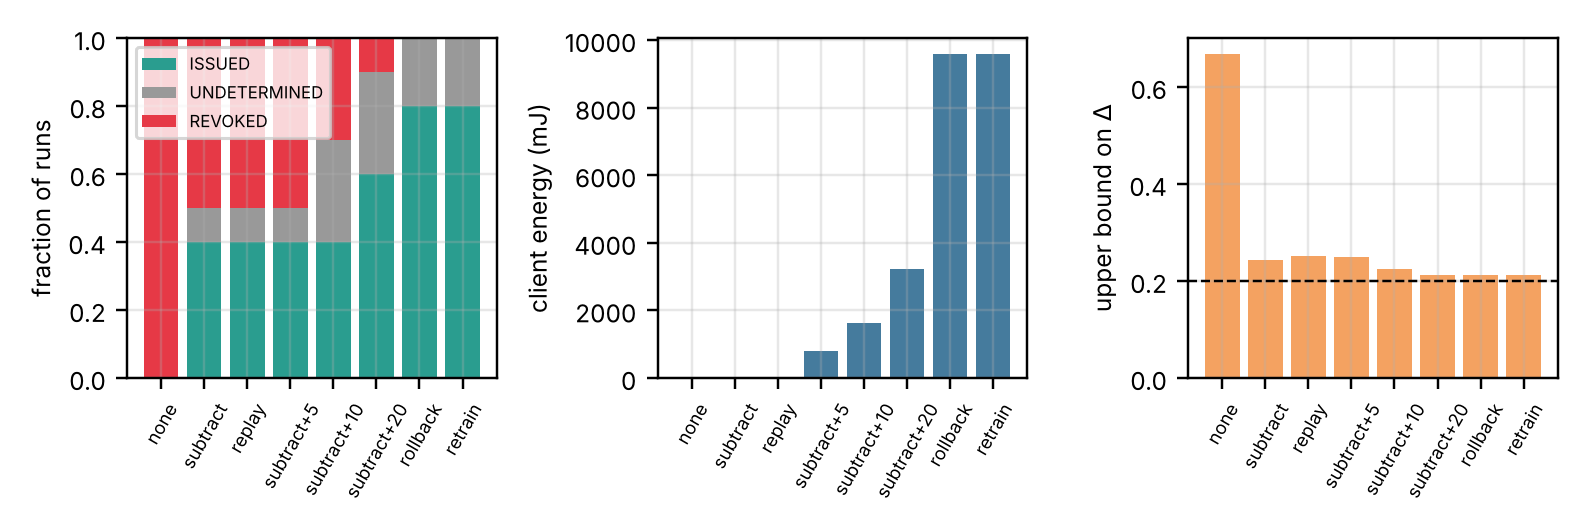
\includegraphics[width=0.92\textwidth]{cert_methods.png}
\caption{Certificate outcomes, client energy and upper confidence bound on the residual advantage per operator (10 seeds). The dashed line is $\epsilon=0.2$.}\label{fig:methods}
\end{figure*}

\subsection{Verify-then-escalate}
The ladder was subtract, subtract+5, subtract+20, rollback, each tested at $\alpha/4$, with a validation set of 300 samples and a 3-point accuracy guard. It certified 10 of 10 waves at accuracy 0.98, against 8 of 10 for always retraining at the full level. It released subtract+5 four times, subtract+20 twice and rollback four times. Mean client energy was 6.6~J against 9.6~J for retraining (31\% less, 41 instead of 60 rounds on average), but the cost is bimodal: from 0.8~J when the first rung succeeded to 13.8~J, 44\% above retraining, when all four rungs were tried because failed attempts are paid for. Fixing subtract+5 as the only operator was cheapest (0.8~J) and was certified in 4 of 10 runs only (Fig.~\ref{fig:esc}).

\begin{figure}[t]
\centering
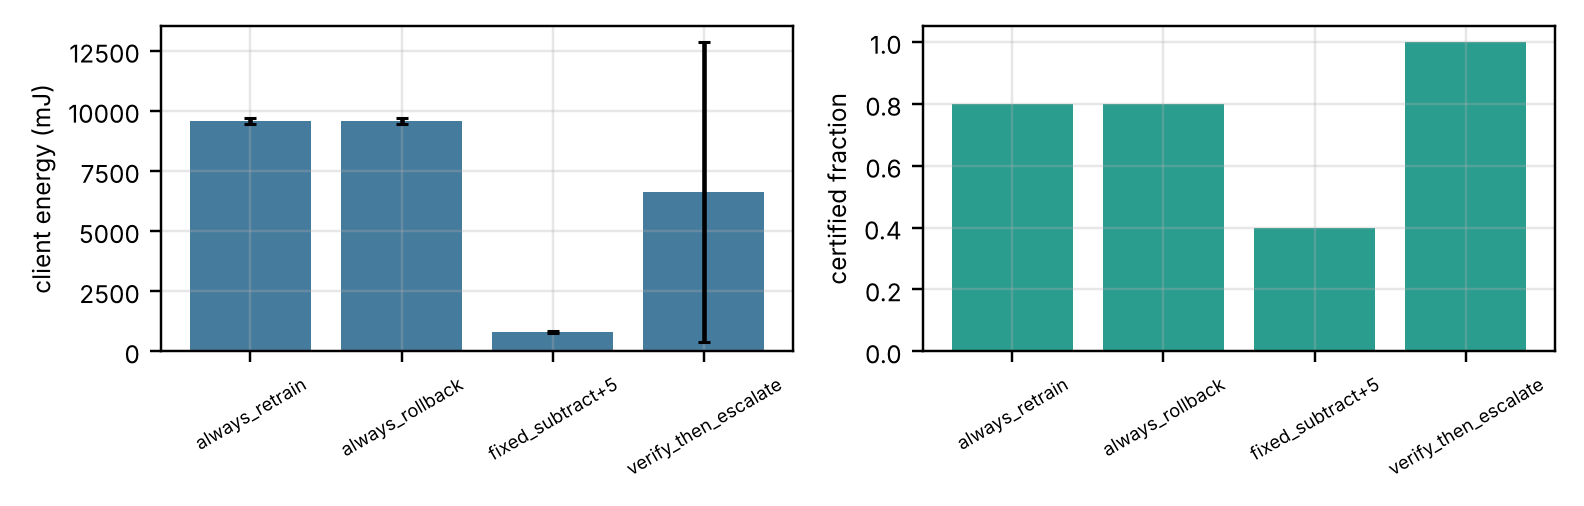
\includegraphics[width=\columnwidth]{cert_escalation.png}
\caption{Policies on the same waves: mean client energy (error bars: s.d.) and fraction of waves certified.}\label{fig:esc}
\end{figure}

\subsection{Wave size and batching}
Retraining cost per revoked client falls from 3.4~J for waves of 4 to 0.24~J for waves of 30, because rollback cost does not grow with the wave (Fig.~\ref{fig:wave}). Serving 20 requests one at a time costs 14.0~J each (measured on three requests and extrapolated), 29 times more than a single batched wave. The price is delay and the need for enough pairs: the retrained model was certified in 3 of 5 runs at $W{=}4$ (24 pairs) and in 5 of 5 at $W\in\{8,20,30\}$, with 4 of 5 at $W{=}12$. Revealing the canaries sends $2m(d{+}1)\cdot 4$ bytes per client, 0.98~MB for $W{=}20$. In practice requests have to be held until a wave is large enough, which is compatible with the response periods of data protection law but should be agreed with the regulator.

\begin{figure}[t]
\centering
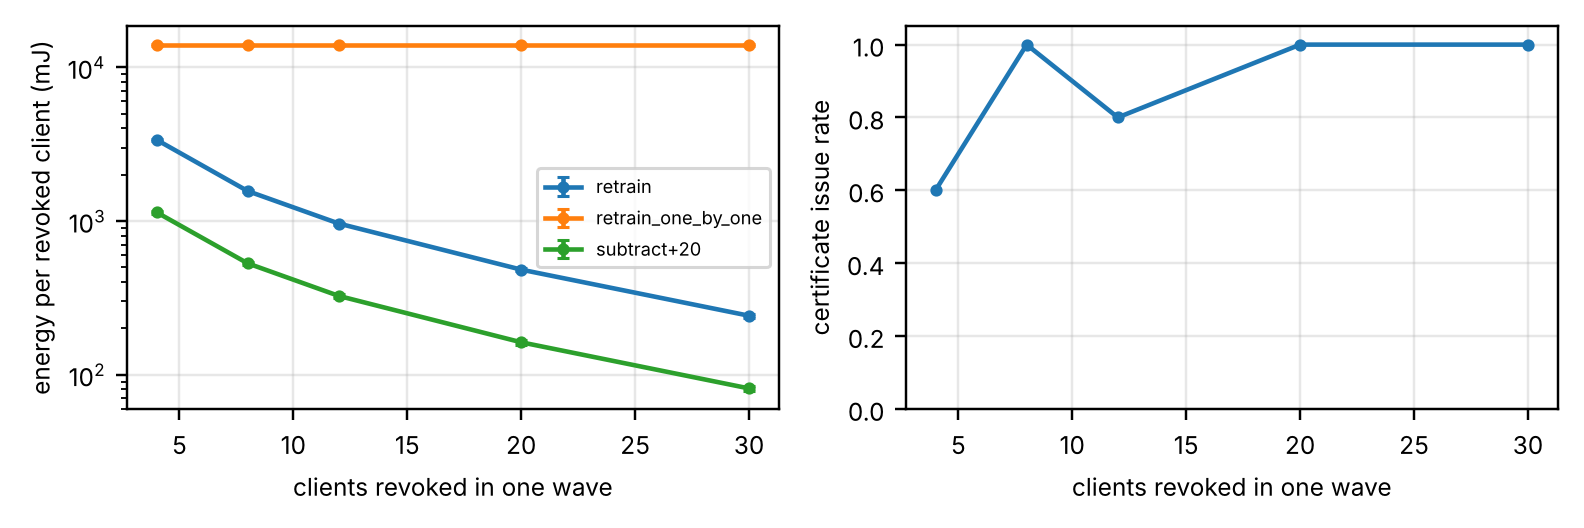
\includegraphics[width=\columnwidth]{cert_wave.png}
\caption{Energy per revoked client versus wave size (left) and issue rate for the retrained model (right, 5 seeds).}\label{fig:wave}
\end{figure}

\subsection{Poisoned and Byzantine clients}
Three or eight clients in the wave stamped a trigger on half of their data (relabelled to the target class); in half of the runs 12 further clients were Byzantine sign-flippers. Before unlearning the backdoor attack success rate was 0.29 with three poisoned clients and 0.71 with eight (0.31 and 0.71 with Byzantine clients present). After subtraction with 10 recovery rounds it fell to 0.007 and 0.002 (0.016 and 0.010 with Byzantine clients), against 0.027 for retraining and 0.029 for a model never trained on them, at 2.1--2.3~J versus 12.5--13.8~J, with accuracy unchanged (Fig.~\ref{fig:poison}). The rate of the clean model is the false-trigger floor. Recovery was as effective with the Byzantine clients present.

\begin{figure}[t]
\centering
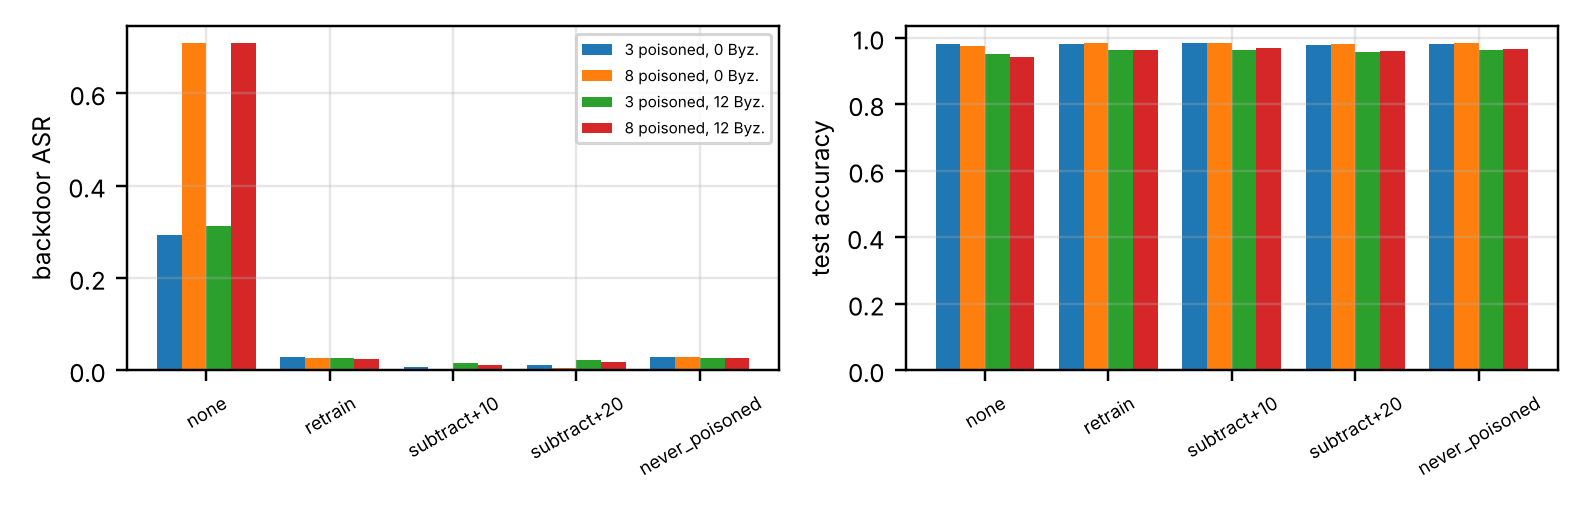
\includegraphics[width=\columnwidth]{cert_poison.png}
\caption{Backdoor success rate and test accuracy before and after unlearning, with 3 or 8 poisoned clients and 0 or 12 Byzantine clients (5 seeds).}\label{fig:poison}
\end{figure}

\subsection{Heterogeneity, participation, noise and capacity}
Fig.~\ref{fig:sweeps} shows the bound for the un-unlearned model and for three operators over four factors (5 seeds). The approximate operators were certified more often with stronger heterogeneity (subtract+10: 5, 2 and 3 of 5 runs at $\alpha=0.1,1,10$), lower participation (4, 2 and 3 of 5 at $p=0.3,0.6,1$) and more DP noise (2 and 5 of 5 at $\sigma=0$ and $0.02$). We did not isolate the cause; fewer exposures of a canary and noise on the update both plausibly reduce what the model retains. Accuracy fell with noise (0.98 to 0.94 at $\sigma=0.02$) for every operator. Capacity matters for audit power: at $d=64$ the un-unlearned model was certified in 3 of 5 runs, because the model cannot memorise the canaries, so the advantage really is below $\epsilon$ there; at $d\ge 256$ it was flagged in all runs.

\begin{figure}[t]
\centering
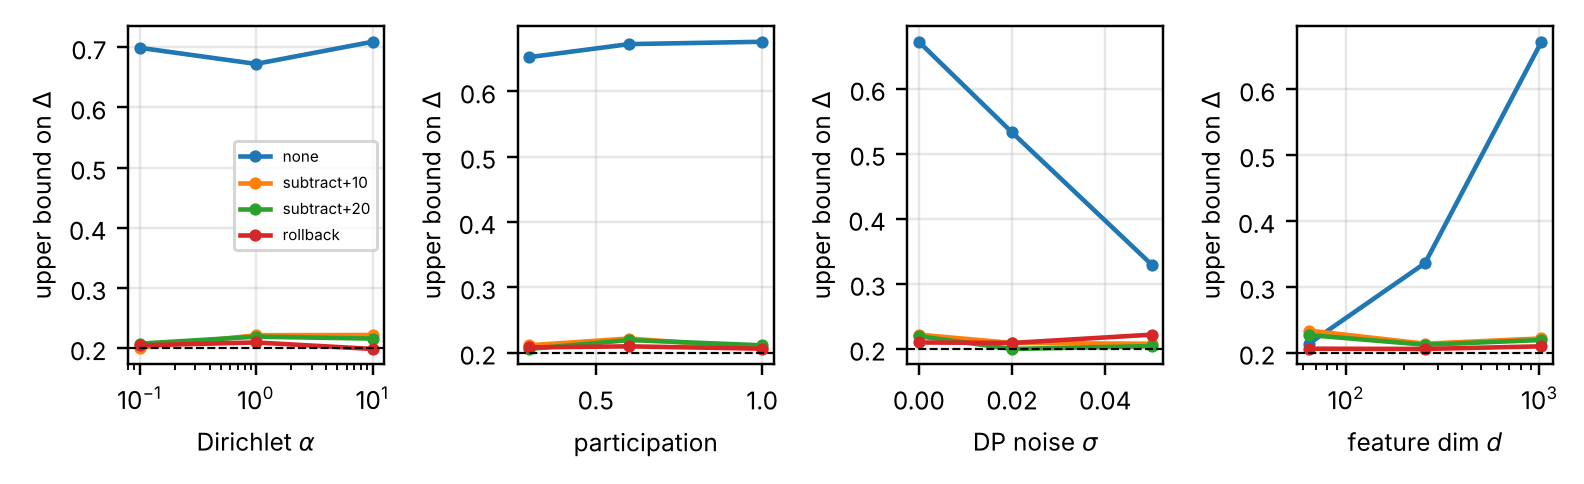
\includegraphics[width=\columnwidth]{cert_sweeps.png}
\caption{Upper bound on the residual advantage versus Dirichlet $\alpha$, participation, DP noise and feature dimension (5 seeds). Dashed: $\epsilon=0.2$.}\label{fig:sweeps}
\end{figure}

\subsection{Provenance overhead and tamper detection}
For 60 rounds the ledger holds 61 records and 101~kB (1.7~kB per round), about 1.1\% of update upload traffic. Verifying the whole chain took 1.6~ms and a Merkle inclusion proof (5--6 hashes) about 5~$\mu$s. In 3 seeds $\times$ 200 random edits of a record field (root, model hash, round, weights, flagged list), the chain check detected all 600; an HMAC-signed certificate failed on any change of its status; a forged rollback record that kept training the revoked wave was rejected by the lineage audit; and the lineage audit passed for every operator in the main experiment. The server's checkpoints took 417~kB, but stored updates 15.2~MB, which is the main storage cost of the cheap operators.



\subsection{Real IoT data and a nonlinear model}
\textbf{Data and setup.} UCI HAR~\cite{anguita2013} gives 561 smartphone inertial features for 30 subjects, one client per subject (natural non-IID split; task: dynamic versus static activity). N-BaIoT~\cite{meidan2018} gives 115 traffic statistics from nine commercial IoT devices infected with Mirai and BASHLITE; we split each device into five sites with disjoint random subsets of its traffic, giving 45 clients that differ by device type and attack family (task: benign versus attack). Every client keeps 40 records, half benign for N-BaIoT, and plants $m=6$ canary pairs; test records are held out per client. We train a logistic model and a one-hidden-layer MLP (32 tanh units; 18\,049 parameters on HAR, 3\,777 on N-BaIoT), $T=60$, $p=0.6$, and revoke a third of the clients (10 of 30 and 15 of 45; 60 and 90 pairs), 5 seeds, $\epsilon=0.2$. Accuracy is near ceiling (0.997--0.999), so the certificate carries the evidence.

\textbf{Operators.} Table~\ref{tab:har} and Fig.~\ref{fig:har} show the outcomes. The un-unlearned MLP was flagged in 5 of 5 runs on both data sets, and so was the HAR linear model; the N-BaIoT linear model was flagged in 1 of 5, so its audit has no power (116 parameters cannot memorise 270 canaries) and any certificate there is vacuous. Cheap operators were certified about as often as retraining for the MLP on both data sets, but on N-BaIoT plain subtraction cost accuracy for the linear model (0.871 against 0.995) and replay (0.942) too, which is again why the policy has a utility guard. With 60 to 90 pairs the test is near its resolution: retraining was certified in 3 to 5 of 5 runs. The MLP is expensive on the device: retraining costs 86.5~J on HAR against 2.7~J for the linear model, and 27.4~J on N-BaIoT.

\begin{table}[t]
\centering
\caption{Certificate outcomes I/U/R (issued, undetermined, revoked) on real data, wave of one third of the clients, 5 seeds.}\label{tab:har}
\footnotesize
\begin{tabular}{@{}lcccc@{}}
\toprule
 & \multicolumn{2}{c}{HAR} & \multicolumn{2}{c}{N-BaIoT}\\
Operator & Linear & MLP & Linear & MLP\\
\midrule
none & 0/0/5 & 0/0/5 & 3/1/1 & 0/0/5\\
subtract & 2/2/1 & 3/2/0 & 4/1/0 & 5/0/0\\
replay & 2/1/2 & 3/2/0 & 4/1/0 & 4/1/0\\
subtract+5 & 2/2/1 & 4/1/0 & 4/1/0 & 5/0/0\\
subtract+10 & 2/2/1 & 4/1/0 & 4/1/0 & 4/1/0\\
subtract+20 & 3/1/1 & 4/1/0 & 4/1/0 & 5/0/0\\
retrain & 3/2/0 & 4/1/0 & 4/1/0 & 5/0/0\\
\bottomrule
\end{tabular}
\end{table}

\begin{figure*}[t]
\centering
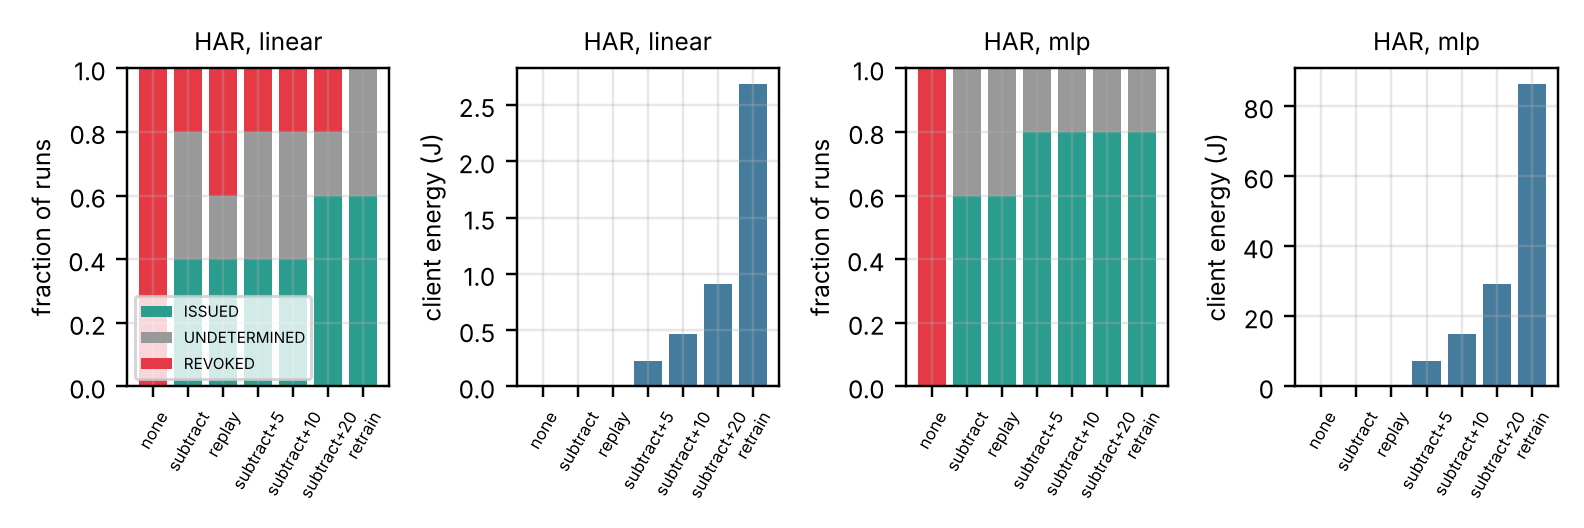
\includegraphics[width=0.92\textwidth]{har_methods.png}
\caption{UCI HAR: certificate outcomes and client energy per operator for the linear model and the MLP (5 seeds).}\label{fig:har}
\end{figure*}

\textbf{Calibration and the power check.} Over 280 exactly retrained models (synthetic 40; HAR linear and MLP 60 each; N-BaIoT linear and MLP 60 each) the verifier flagged 4 (1.4\%: 2 on HAR with the MLP, 2 on N-BaIoT with the linear model), below the level $\alpha=5\%$. The un-unlearned model was flagged in 160 of 160 runs on the synthetic fleet and on HAR, but in only 35 of 60 runs for the N-BaIoT MLP at $T=30$ and 9 of 60 for its linear model; in the remaining runs the model had not memorised the canaries enough, so the certificate that follows is true but says little. The policy therefore audits the model before unlearning and reports \textsc{unpowered} instead of \textsc{issued} when it is not flagged: on the N-BaIoT linear model it did so in 3 of 5 waves. For the MLP on N-BaIoT the ladder certified 5 of 5 waves at 0.88~J against 27.4~J for retraining (97\% less; 2 rounds on average; accuracy 0.982 against 0.997), and on HAR it certified the same waves as retraining at 1.7~J against 2.7~J (linear) and 25.6~J against 86.5~J (MLP).

\textbf{Poisoning.} On N-BaIoT a trigger stamped on the first three features of half of the records of 2 or 5 clients implanted: the attack success rate before unlearning was 0.25 and 0.45 for the linear model and 0.36 and 0.59 for the MLP. Subtraction with 10 recovery rounds reduced it to 0.003--0.010, against 0.007--0.020 for retraining and 0.009--0.030 for a model never trained on them, at 0.2~J instead of 1.3~J (linear) and 6.6~J instead of 39.3~J (MLP, 2 poisoned clients), with accuracy unchanged. On HAR the same kind of trigger did not implant (attack success at most 7\% even with triggers on up to 60 features, $8\sigma$, 10 of 30 clients), because the sensor features separate the classes too strongly, so HAR is not informative about poisoning.

\textbf{Per-client certificates.} A wave of one client has only $m$ pairs. On HAR with the MLP and $m=60$, the un-unlearned model was flagged in 5 of 5 runs and the retrained model certified in 5 of 5 at $\epsilon=0.2$ (subtract+20 in 4 of 5); at $m=40$ retraining was certified in 3 of 5, and at $\epsilon=0.3$, $m\ge 40$ sufficed (Fig.~\ref{fig:perclient}). On N-BaIoT the audit had no power at this model size: with $m=60$ the un-unlearned MLP was flagged in 0 of 5 runs and with $m=100$ in 1 of 5, and widening the hidden layer to 128 units (15\,000 parameters) raised this only to 2 of 5. Canaries are 60\% of a device's records ($m{=}60$), raising local compute 2.5 times, small beside the radio cost, and they use up capacity: the linear HAR model, with 562 parameters, was flagged in 3 of 5 runs at $m=100$ against 4 of 5 at $m=40$. Per-client certificates therefore need a model with spare capacity relative to the canary budget, and the power check shows when that is not the case.

\begin{figure}[t]
\centering
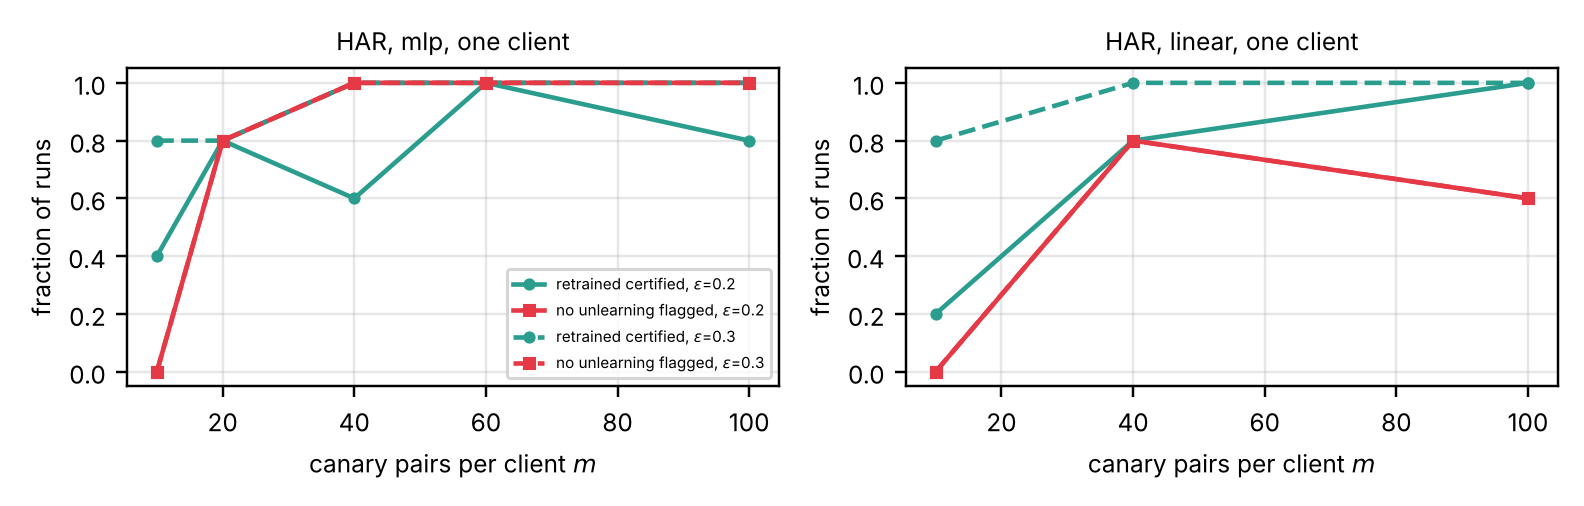
\includegraphics[width=\columnwidth]{har_per_client.png}
\caption{One revoked client on UCI HAR: share of runs in which the retrained model is certified and the un-unlearned model is flagged, against the number of canary pairs per client (5 seeds).}\label{fig:perclient}
\end{figure}

\section{Discussion and Limitations}
\label{sec:disc}
\textbf{What a certificate means.} It bounds the advantage that two declared scores extract from the canary cohort of the wave on the released model, and holds at any stopping time. It is not erasure in parameter space, and it does not cover attacks outside the score class. Canaries must be planted before training, so models trained without them cannot be certified retroactively, and a provider that treats canary records specially defeats the audit. The ledger audit certifies lineage only; the statistical certificate and the lineage check answer different questions and both are reported.

\textbf{Limits of the evidence.} The data are a synthetic fleet and two real data sets (UCI HAR, whose classes are easy to separate, and N-BaIoT, in which we split each device into five sites ourselves), with a linear model and a one-hidden-layer MLP, 5--10 seeds, simulated clients and a modelled energy cost. We have not run deeper networks, other IoT modalities or measured device energy, and the audit's power depends on the model's capacity to memorise: it was weak for the N-BaIoT models, which is why the policy reports \textsc{unpowered} audits. A certificate is issued per wave; certifying one client alone needed about 60 canary pairs and a model with spare capacity (HAR MLP, not N-BaIoT), and the canaries take up most of a small device buffer. The audit tests canaries, which are random records; a cheap operator can remove the influence of those and still leave subtle influence of real records, which the canary test cannot see. This is why plain subtraction was certified on HAR at no client energy, and the certificate should not be read as proof about real-sample membership. The escalation policy saves energy on average but can cost more than retraining in the worst case, so a deployment should cap the number of attempts. Sample- and class-level requests are implemented for rollback and retraining but neither tested nor evaluated here, and feature-level forgetting is not supported.

\textbf{Regulatory alignment.} The ledger and the certificate give a data controller a verifiable record that a revocation was honoured; whether this satisfies a specific legal duty is a question for counsel, and we make no such claim.

\section{Conclusion}
We combined a hash-chained provenance ledger, per-round state checkpoints, paired-canary e-process certificates and a cost ladder into a federated unlearning workflow whose acceptance test is statistical rather than empirical. On a synthetic fleet, smartphone sensor data and botnet traffic from nine IoT devices, with a linear model and an MLP, the audit wrongly flagged an exactly retrained model in 1.4\% of runs, below its 5\% level, and flagged the un-unlearned model whenever the canaries were memorised; where they were not, the power check said so. The ladder certified waves at 31 to 97\% lower mean energy than retraining, and batching revocations cut per-client cost by an order of magnitude. A single client could be certified with 60 canary pairs on a HAR MLP. Next steps are deeper networks, other IoT modalities, measured device energy, a canary design that tests real records, and attacks that adapt to the audit.

\bibliographystyle{IEEEtran}
\bibliography{refs}
\end{document}
